\documentclass[11pt,a4paper]{article}
\usepackage[T1]{fontenc}
\usepackage[utf8]{inputenc}
\usepackage{lmodern}
\usepackage[a4paper,margin=27mm,headheight=15pt]{geometry}
\usepackage{amsmath,amssymb,amsthm,mathtools}
\usepackage{microtype,booktabs,array,graphicx,xcolor,enumitem}
\usepackage{fancyhdr}
\usepackage[colorlinks=true,linkcolor=blue!45!black,citecolor=blue!45!black,
  urlcolor=blue!45!black,breaklinks=true]{hyperref}
\usepackage[nameinlink,noabbrev]{cleveref}
\numberwithin{equation}{section}
\newtheorem{theorem}{Theorem}[section]
\newtheorem{lemma}[theorem]{Lemma}
\newtheorem{proposition}[theorem]{Proposition}
\newtheorem{corollary}[theorem]{Corollary}
\theoremstyle{definition}
\newtheorem{definition}[theorem]{Definition}
\newtheorem{example}[theorem]{Example}
\theoremstyle{remark}
\newtheorem{remark}[theorem]{Remark}
\setlist[enumerate]{leftmargin=*,itemsep=3pt,topsep=5pt}
\setlist[itemize]{leftmargin=*,itemsep=3pt,topsep=5pt}
\setlength{\emergencystretch}{2em}
\pagestyle{fancy}
\fancyhf{}
\fancyhead[L]{\small Positive prime signals and zero cancellation}
\fancyhead[R]{\small Research note}
\fancyfoot[C]{\thepage}
\renewcommand{\headrulewidth}{0.3pt}
\hypersetup{pdftitle={Positive prime signals and optimal zero cancellation},
 pdfauthor={Research note prepared for Vladimir Reshetnikov},
 pdfsubject={Two extensions of the supplied Dirichlet GRH research collection}}

\title{\bfseries Positive prime signals and\protect\\optimal zero cancellation\\[5pt]
\large Two extensions of the supplied Dirichlet GRH research collection}
\author{Research note prepared for Vladimir Reshetnikov}
\date{27 November 2026}

\begin{document}
\maketitle
\begin{abstract}
We develop two extensions of the supplied research collection, using the
Dirichlet GRH theorem exported by \texttt{lsernau/grh-lean} as the arithmetic
input. First, an explicitly computable real weight, uniformly as close to
one as desired, makes the autocorrelation of one smoothed prime signal
determine every labelled primitive Dirichlet zero multiset, including
orientation and multiplicity. This answers an explicit question in the
collection. The construction combines its positive algebraic prefix code
with three bounded modulations and an irrational-reflection argument;
the latter has established phase-retrieval antecedents. Second, we give a
complete positive-measure treatment of the shortest average annihilating
two prescribed frequencies and prove an asymmetric cube-root resonance law,
together with sharp stability and a shortening coefficient. The
optimization has classical input-shaping antecedents, which are credited;
the proposed refinement is the quantified resonance and stability analysis.
All mathematical proofs are included. Numerical and exact-arithmetic
artifacts check the constructions but are not formal proof certificates.
\end{abstract}

\vspace{3pt}
\noindent\textbf{Status.} Complete human-readable proofs; independent
analytic review within this research run; no new Lean kernel verification.
Novelty is assessed relative to the pinned collection and a targeted
literature search, with historical-priority limits stated explicitly.

\tableofcontents
\newpage
\section{What was inspected, and where the new work begins}

\subsection{Pinned sources and the proved scope}

The upstream source is \texttt{lsernau/grh-lean} \cite{GRHLean},
pinned at commit
\begin{center}
\texttt{72fead102f663d5c7a407964a13dc0cf9d977207}.
\end{center}
The companion source is the merged article in
\texttt{VladimirReshetnikov/ProveIt} \cite{ProveItArticle}, pinned at commit
\begin{center}
\texttt{22e5c8b7dda558fd9a50b61465483cb4c0433694}.
\end{center}
These references identify the material used here, even if either
repository subsequently changes.

The upstream \texttt{Statements.lean} imports Mathlib alone. Its types
are about Mathlib's Riemann zeta function and Dirichlet $L$-functions.
The five results exported by \texttt{Main.lean} include
\texttt{riemannHypothesis} and
\texttt{LFunction\_eq\_zero\_re}, the latter asserting that every
Dirichlet zero in the open critical strip has real part $1/2$.
The main statements do not assume a substitute analytic inequality as an
extra premise. The scope is RH and GRH for Dirichlet characters; statements
about general Artin or automorphic $L$-functions do not follow merely by
changing the name of the family.

Andrew Sutherland's primary verification record, updated on 27 November
2026, reports successful builds, statement comparisons, axiom audits and
independent kernel checks for both editions at this commit
\cite{Sutherland2026}. The recorded axiom dependencies are
\texttt{propext}, \texttt{Classical.choice} and \texttt{Quot.sound}.
Our work inspected the pinned source, the exported statements and the
main reduction, and performed a source scan. We did not independently
rebuild the upstream Lean development. Published kernel checks and this
source review are different pieces of evidence.

\subsection{The transferable mechanism}

The source's central comparison combines sufficiently many short forms
with a lower bound on the size of integral forms. The determinant and
product formula enforce a schematic estimate
\[
 m\,\mathrm{remainder}\le f a(\log b)^5,
 \qquad m\asymp\sqrt{x}.
\]
Its arithmetic reduction gives a one-sided estimate of the shape
\[
 R_{q,d}(x)\le x^{-1/2+\eta}\quad\text{eventually for every }\eta>0,
\]
for a smoothed prime-power remainder carrying a quadratic-character
weight. The final analytic argument is explicit in
\texttt{New/Reduction/Zeros}: the transformed remainder has residues
given by differences of zero multiplicities, an auxiliary twist avoids
the specified zero region, and a Landau sign argument excludes zeros to
the right of the critical line. Functional equations finish the reduction.
The reading guide and the proof files describe this chain
\cite{GRHLean}.

We use the proved zero-location theorem and its positive spectral
consequences. We do not presume that the source's deep determinant
construction transfers unchanged to a new family. The additional
arguments in this note are harmonic analysis, convexity, algebraic
separation and explicit-formula analysis, proved below.

\subsection{The precise additions to the collection}

The merged article describes itself as a synthesis of 103 reports,
containing 760 results in 621 pages; it also explicitly says that the
merge was not an independent mathematical review \cite{ProveItArticle}.
All its section source files were retrieved, and the relevant inverse
and filter sections were read in detail. The following comparison fixes
the contribution of the present work.

\begin{center}
\small
\begin{tabular}{@{}p{.30\linewidth}p{.31\linewidth}p{.31\linewidth}@{}}
\toprule
Question & Existing result & Addition proved here\\
\midrule
One real nonnegative weight & One complex weight encodes all labelled
Dirichlet zero spectra & One real positive weight does so, with a known
prime-only correction, and may be arbitrarily close to one\\[4pt]
Nonconsecutive zero frequencies & Sharp single-frequency jets and
consecutive-harmonic averages & Every pair of frequencies; all
minimizers; cube-root versus linear resonance asymptotics; exact
shortening slope\\
\bottomrule
\end{tabular}
\end{center}

The arithmetic result uses exact limiting data. It is not a claim that a
finite noisy measurement can recover infinitely many zeros. Its novelty
lies in the positive real prime-side construction and the recovery of
the labelled oriented spectra. The underlying irrational-reflection
mechanism is related to established phase-retrieval results
\cite{Liehr2024,Wellershoff2024}.

The filter problem is also the undamped positive two-mode input-shaping
problem from vibration control. The low-ratio formula, and numerical
descriptions of simultaneous two-mode shapers, have older precedents
\cite{Singhose1997,Crain1996}. We therefore do not claim that positive
two-frequency cancellation was introduced here. The quantitative
resonance theorem and its shortening and stability consequences are
the proposed new refinement. The supplied collection does not contain
these two extensions. A targeted search cannot certify worldwide
historical priority; the proofs stand independently of that question.

\subsection{A reading route}

For the main arithmetic theorem, start with
Theorem~\ref{rw:thm:encoder}, then follow the coefficient formula
\eqref{rw:eq:weight}, the amplitude recovery
\eqref{rw:eq:decodeA}, and the terminating reflection reconstruction
\eqref{rw:eq:Pelltelescope}. For the extremal theorem, start with
Theorems~\ref{filt:classification} and~\ref{filt:cusp}.
The nonnegative function in~\eqref{filt:g} is the certificate that
no shorter positive average can work. Appendix~\ref{app:verification}
describes the reproducible checks and the exact scope of verification.

\clearpage
\part{A positive real arithmetic signal}
% Self-contained mathematical section. Requires amsmath, amssymb, amsthm.
% Bibliography keys: ProveItArticle, GRHLean, Liehr2024, Wellershoff2024.
\section{One positive prime weight determines all labelled Dirichlet zeros}
\label{rw:sec:main}

The inverse-problem section of the supplied article constructs a complex
prime weight whose autocorrelation determines all labelled primitive
Dirichlet zero multisets. It asks whether one real nonnegative weight can
do the same \cite[section ``Recovering zeros and characters from prime
data'', final question ``Fewer filters and weights'']{ProveItArticle}.
The answer below is affirmative. Second-order correlation already suffices.
The weight is computable independently of the zeros and stays uniformly
close to one. The construction uses three bounded frequency shifts to
recover the orientation that taking real parts would otherwise erase.

Throughout this section, Dirichlet GRH means that the nontrivial zeros of
every primitive Dirichlet $L$-function lie on $\Re s=1/2$. This is exactly
the input supplied by the main exported theorems of \cite{GRHLean}; no
hypothesis about Artin or automorphic $L$-functions is used. Put
\[
 m_\chi(t)=\operatorname{ord}_{s=1/2+it}L(s,\chi),\qquad
 D(t)=(\tfrac12+it)(\tfrac32+it),\qquad
 K(t)=|D(t)|.
\]
At a nonzero value of $L$, the order is zero. Write $m_\zeta$ for the
conductor-one character. Both signs of $t$ are retained for a nonreal
character.

\begin{theorem}[A real positive universal arithmetic encoder]
\label{rw:thm:encoder}
There is an explicitly specified computable function
$W:\mathbb N_{\ge1}\to[3/4,5/4]$, independent of the zero multisets, such that the
following holds under Dirichlet GRH. Define, for real $t$,
\[
 F(t)=e^{-t/2}\left\{
 \sum_{1\le n\le e^t}\Lambda(n)W(n)(1-ne^{-t})-\frac{e^t}{2}\right\}.
\]
The real autocorrelation
\[
 C(h)=\lim_{T\to\infty}\frac1T\int_0^T F(t+h)F(t)\,dt
 \qquad(h\in\mathbb R)
\]
exists, is continuous, even and positive definite, and determines
$m_\chi(t)$ for every primitive character $\chi$ and every real $t$.
In particular, the labels, multiplicities and signs of the ordinates are
recovered. No simplicity, common-zero exclusion or linear independence
assumption is required.

The same conclusion holds for a sum over primes alone after adding the
explicit bounded correction in Corollary~\ref{rw:cor:primes}.
More generally, for every prescribed rational $0<\varepsilon<1$ one
can require $1-\varepsilon\le W(n)\le1+\varepsilon$ for all $n$.
The determination uses exact limiting correlation data. It does not
assert a uniformly stable reconstruction from a fixed finite observation.
\end{theorem}

\subsection{A separated positive code}

Enumerate all pairs $(\chi_j,a_j)$, where $\chi_j$ is primitive and
nonprincipal and $a_j\in\{0,1,\sqrt2\}$, as $j=1,2,\ldots$, in a fixed
computable order. For example, order the characters by conductor and then
by their finite tables of algebraic values, and list the three shifts
consecutively. Let $q_j$ be the conductor and $w_j=q_j+1$. Put $c_0=1$,
$w_0=2$, $k_0=0$, and let $p_j$ denote the $j$th rational prime.
The construction below is the multiquadratic prefix code of
\cite[lemma ``Prefix separation'']{ProveItArticle}, with a smaller tail
budget needed for a real positive weight. It is included in full.

Inductively set
\begin{align}
 D_n^*&=2^{\max_{0\le j\le n}k_j},&
 d_n&=(D_n^*)^{-1}
       \bigl(3D_n^*(n+1)\bigr)^{-(2^n-1)},\label{rw:eq:dn}\\
 c_j&=2^{-k_j}\sqrt{p_j},\label{rw:eq:cj}
\end{align}
where $k_j$ is the least nonnegative integer satisfying
\begin{equation}\label{rw:eq:codechoice}
 2^{-k_j}p_jw_j\le
 2^{-j-3}\min\left(1,\min_{0\le n<j}\frac{d_n}{n+1}\right).
\end{equation}
Every comparison in \eqref{rw:eq:codechoice} is rational, so the choice is
effective. In particular $d_0=1$, and
\begin{equation}\label{rw:eq:tails}
 \sum_{j\ge1}c_jw_j\le\frac18,\qquad
 \sum_{j>n}c_jw_j\le
 2^{-n-3}\frac{d_n}{n+1}.
\end{equation}

\begin{lemma}[Prefix decoding]\label{rw:lem:code}
If $u_0,\ldots,u_n$ are integers, not all zero, with
$|u_j|\le(n+1)w_j$, then
\[
 \left|\sum_{j=0}^n c_ju_j\right|\ge d_n.
\]
Consequently $E(m)=\sum_{j\ge0}c_jm_j$ is injective on nonnegative integer
sequences satisfying $m_j\le H w_j$ for some finite $H$.
If $n+1\ge H$ and $|A'-E(m)|<d_n/8$, the true prefix is the unique vector
of integers $0\le v_j\le(n+1)w_j$, $0\le j\le n$, satisfying
\[
 \left|A'-\sum_{j=0}^n c_jv_j\right|<\frac{d_n}{2}.
\]
\end{lemma}

\begin{proof}
The field $\mathbb Q(\sqrt{p_1},\ldots,\sqrt{p_n})$ has degree $2^n$;
its automorphisms change the signs of the square roots independently.
The square classes of the distinct primes are independent, as follows
by taking their valuations modulo two. Thus
$z=D_n^*\sum_{j=0}^nc_ju_j$ is a nonzero algebraic integer. Every conjugate
of $z$ has modulus at most
\[
 D_n^*(n+1)\left(w_0+\sum_{j=1}^nc_jw_j\right)
 \le\frac{17}{8}D_n^*(n+1)<3D_n^*(n+1).
\]
The product of its $2^n$ conjugates is a nonzero integer. Bounding all
but the displayed conjugate gives precisely the lower bound $d_n$.
By \eqref{rw:eq:tails}, the omitted tail of $E(m)$ is at most $d_n/8$
when $n+1\ge H$. The true prefix is therefore within $d_n/4$ of $A'$;
every other admissible prefix is more than $3d_n/4$ away. Finally, if two
sequences differed, a sufficiently long prefix containing a difference
would contradict this uniqueness with $A'=E(m)$.
\end{proof}

Define the promised weight by
\begin{equation}\label{rw:eq:weight}
 W(n)=1+2\sum_{j\ge1}c_j
       \Re\bigl(\chi_j(n)n^{-ia_j}\bigr).
\end{equation}
The series converges uniformly in the positive integer $n$.
Equation~\eqref{rw:eq:tails} gives $|W(n)-1|\le2\sum c_j\le1/4$.
It also gives an effective uniform truncation error, proving the stated
computability of $W$. No zero or zero approximation enters this definition.
For the arbitrary-$\varepsilon$ version, replace $2^{-j-3}$ in
\eqref{rw:eq:codechoice} by $\sigma2^{-j}$, where
$\sigma=\min(\varepsilon/2,1/8)$. All separation and tail estimates remain
valid, while $|W(n)-1|\le2\sigma\le\varepsilon$.

\subsection{The shifted explicit formula and the infinite sum}

\begin{lemma}[Uniformly bounded shifts]\label{rw:lem:explicit}
Assume Dirichlet GRH. Let $\chi$ be primitive and nonprincipal of conductor
$q$, and let $|a|\le\sqrt2$. Uniformly for $x\ge1$,
\begin{equation}\label{rw:eq:shifted}
 \sum_{1\le n\le x}\Lambda(n)\chi(n)n^{-ia}(1-n/x)
 =-\sum_\gamma
 \frac{x^{1/2+i(\gamma-a)}}{D(\gamma-a)}
 +O\bigl(x^{1/4}\log(q+2)\bigr).
\end{equation}
The zeros in this formula are repeated with multiplicity. The implied
constant is absolute, and
\begin{equation}\label{rw:eq:abssum}
 \sum_\gamma |D(\gamma-a)|^{-1}\ll\log(q+2)
\end{equation}
with an absolute constant. For $\zeta$ and $a=0$, the same formula holds
with the additional main term $x/2$.
\end{lemma}

\begin{proof}
We give the uniformity details because they justify using infinitely many
characters. The standard completed function is
\[
 \Xi_\chi(s)=\bigl(s(s-1)\bigr)^{\mathbf1_{q=1}}
 (q/\pi)^{(s+\kappa)/2}\Gamma((s+\kappa)/2)L(s,\chi),
 \qquad \chi(-1)=(-1)^\kappa.
\]
Its Hadamard product and functional equation, with the zeros on the
critical line, give
\begin{equation}\label{rw:eq:poisson}
 \Re\frac{\Xi_\chi'}{\Xi_\chi}(2+iu)
 =\sum_\gamma\frac{3/2}{(3/2)^2+(u-\gamma)^2}.
\end{equation}
For example, subtract the logarithmic derivative at $1/2+iu$, whose real
part is zero away from zeros, and then extend by continuity in $u$.
The Euler series at $2+iu$ and the digamma factor show that the left side
is $O(\log(q(|u|+3)))$, absolutely in $q,u$. Thus each interval
$[u-1,u+1]$ contains $O(\log(q(|u|+3)))$ zeros, with multiplicity.
Summing these estimates over unit intervals proves
\eqref{rw:eq:abssum}, uniformly for the indicated bounded shifts.

For completeness a crude numerical multiplicity bound follows directly.
The digamma series implies
$\Re\psi(x+iy)\le2+\log(|y|+2)$ for $1\le x\le3/2$:
split its series after $N=\lceil\max(2,|y|)\rceil$ terms and bound the
remaining terms by $\tfrac12(n+1)^{-2}+y^2(n+1)^{-3}$.
Also $\sum_{n\ge2}\Lambda(n)n^{-2}<2$ and the two possible rational
terms in $\Xi_\chi'/\Xi_\chi$ have real part at most $3/2$ together.
Hence the left side of \eqref{rw:eq:poisson} is at most
$\tfrac92+\tfrac12\log(q(|u|+3))$. Each zero in $[u-1,u+1]$ contributes
at least $6/13$, so the safe bound
\begin{equation}\label{rw:eq:localcount}
 \#\{\gamma:|\gamma-u|\le1\}
 \le10+2\log(q(|u|+3))
\end{equation}
is valid, including $q=1$.

For $x\ge1$ the Mellin inversion formula is
\[
 \frac1{2\pi i}\int_{(2)}
 -\frac{L'}{L}(s+ia,\chi)\frac{x^s}{s(s+1)}\,ds.
\]
Move the line to $\Re s=1/4$. The logarithmic derivative there is
$O(\log(q(|\Im s|+4)))$, uniformly for $|a|\le\sqrt2$.
To see this bound without proximity to zeros, compare the Hadamard
logarithmic derivative at $1/4+iv$ with that at $2+iv$. The difference
is an absolutely convergent sum of terms bounded by
$O((1+|v-\gamma|^2)^{-1})$; the local count just proved and the elementary
gamma terms give the assertion. Horizontal edges can be chosen at
distance $\gg1/\log(q(T+3))$ from zero ordinates, using the same local
count. Their contributions tend to zero; the resulting logarithmic
derivative bound on these edges is $O(\log^2(q(T+3)))$.
The new vertical integral has absolute value at most
\[
 Cx^{1/4}\int_{\mathbb R}
 \frac{\log(q(|v|+4))}{1+v^2}\,dv
 \ll x^{1/4}\log(q+2).
\]
The crossed poles are at $s=1/2+i(\gamma-a)$, and their residues give
\eqref{rw:eq:shifted}. Nonprincipal characters introduce no pole at
$1-ia$. The poles of the kernel and the trivial zeros have real part
at most zero, so none was crossed. For $\zeta$ with $a=0$, its pole
at $s=1$ contributes $x/2$.
\end{proof}

For each real $\lambda$ put
\begin{equation}\label{rw:eq:amplitude}
 A(\lambda)=m_\zeta(\lambda)+
 \sum_{j\ge1}c_j
 \bigl\{m_{\chi_j}(a_j+\lambda)+m_{\chi_j}(a_j-\lambda)\bigr\}.
\end{equation}
These are nonnegative, and $A(-\lambda)=A(\lambda)$.
The conjugate identity $m_{\bar\chi}(v)=m_\chi(-v)$ is what makes the
second contribution of $2\Re(\chi(n)n^{-ia})$ equal to
$m_\chi(a-\lambda)$.
Since $\sum c_j\log(q_j+2)<\infty$, Lemma~\ref{rw:lem:explicit} and
absolute convergence yield
\begin{equation}\label{rw:eq:Fourier}
 F(t)=G(t)+O(e^{-t/4}),\qquad
 G(t)=-\sum_{\lambda}\frac{A(\lambda)}{D(\lambda)}e^{i\lambda t},
 \qquad
 \sum_\lambda\frac{A(\lambda)}{|D(\lambda)|}<\infty.
\end{equation}
The sum is over the countable union of the shifted spectra and the zeta
spectrum. That union need not be locally finite. Its absolute convergence
is the justification for all regrouping and averaging here; local
finiteness of the union is not assumed.

Expand the absolutely convergent double series for $G(t+h)G(t)$, using
$G$ real. The mean of $e^{i\omega t}$ is zero unless $\omega=0$.
The decaying error in \eqref{rw:eq:Fourier} does not change the mean.
Consequently
\begin{equation}\label{rw:eq:correlation}
 C(h)=\sum_\lambda\frac{A(\lambda)^2}{K(\lambda)^2}e^{i\lambda h}.
\end{equation}
This is an absolutely convergent series with nonnegative Fourier
coefficients, proving the existence and the stated properties of $C$.
Its Fourier--Bohr coefficients are
\begin{equation}\label{rw:eq:decodeA}
 P(\lambda):=\lim_{U\to\infty}\frac1U\int_0^U
 C(h)e^{-i\lambda h}\,dh
 =\frac{A(\lambda)^2}{K(\lambda)^2},\qquad
 A(\lambda)=K(\lambda)\sqrt{P(\lambda)}.
\end{equation}
Here the positive square root is justified by the nonnegative amplitudes.
At $\lambda=0$ the same formula holds without an extra factor of two.

Equation~\eqref{rw:eq:localcount} implies that the integer vector
\[
 \bigl(m_\zeta(\lambda),
 m_{\chi_j}(a_j+\lambda)+m_{\chi_j}(a_j-\lambda)\ (j\ge1)\bigr)
\]
satisfies the bound in Lemma~\ref{rw:lem:code}. One explicit sufficient
choice is
\begin{equation}\label{rw:eq:Hlambda}
 H_\lambda=\left\lceil30+10\log(|\lambda|+5)\right\rceil.
\end{equation}
Indeed each paired multiplicity is at most
$20+4\log(q_j(|\lambda|+5))\le H_\lambda(q_j+1)$, using
$\log q\le q-1$; the zeta coordinate is smaller than $2H_\lambda$.
The prefix code therefore recovers, for every character, the three
functions
\begin{equation}\label{rw:eq:Sa}
 S_{\chi,a}(x)=m_\chi(a+x)+m_\chi(a-x),
 \qquad a=0,1,\sqrt2.
\end{equation}

\subsection{Recovering an oriented discrete spectrum from reflections}

The reflection principle used next has close precedents in holomorphic
phase retrieval. Liehr characterizes parallel-line uniqueness by exclusion
of an arithmetic progression \cite{Liehr2024}, and Wellershoff treats
three parallel lines with rationally independent distances
\cite{Wellershoff2024}. We include the elementary discrete-measure
argument and an exact stopping rule; the reflection principle itself is
not asserted to be new.

\begin{proposition}[The reflection-group criterion]
\label{rw:prop:reflection}
Let $\mathcal A\subset\mathbb R$ be nonempty and let $a_0\in\mathcal A$.
For locally finite positive atomic measures, the family of centered
symmetrizations about $a\in\mathcal A$ is injective if and only if
\[
 \Gamma=\left\langle2(a-a_0):a\in\mathcal A\right\rangle_{\mathbb Z}
\]
is nondiscrete. In particular, three centers $a_0,a_1,a_2$ with
$(a_1-a_0)/(a_2-a_0)$ irrational suffice, whereas two centers never
suffice for all locally finite positive atomic measures.
\end{proposition}

\begin{proof}
If two measures have the same symmetrizations, their signed difference
$\nu$ satisfies $R_a\nu=-\nu$, where $R_a$ is reflection about $a$.
Composing two reflections gives invariance under every translation in
$\Gamma$. A nondiscrete additive subgroup of $\mathbb R$ is dense.
If $\nu$ had a nonzero atom, translation would give equal nonzero atoms
at a dense set of translates. Infinitely many would lie in one compact
interval, contradicting local finiteness of its total variation.
Since $\nu$ is atomic, it is zero.

Conversely, a discrete subgroup is either $b\mathbb Z$ for $b>0$, or
$\{0\}$. In the first case choose $0<\delta<b/2$ and set
\[
 \mu=\sum_{k\in\mathbb Z}\delta_{a_0+\delta+kb},\qquad
 \widetilde\mu=\sum_{k\in\mathbb Z}\delta_{a_0-\delta+kb}.
\]
These are distinct and every reflection $R_a$, $a\in\mathcal A$,
interchanges them because $2(a-a_0)\in b\mathbb Z$.
Their symmetrizations therefore agree. For $\Gamma=\{0\}$ use the
two single atoms at $a_0\pm\delta$. The lattice counterexamples have
bounded multiplicities and finite $(1+t^2)^{-1}$-weighted mass. They
are abstract spectra, not asserted Dirichlet zero multisets.
\end{proof}

For Dirichlet zeros one can recover each multiplicity by a terminating
finite calculation once exact values of the symmetrizations are supplied.
Let $m:\mathbb R\to\mathbb Z_{\ge0}$ have locally finite support and set
$S_a(x)=m(a+x)+m(a-x)$. Define
\begin{equation}\label{rw:eq:Da}
 \Delta_a(y)=S_a(y+a)-S_0(y)=m(y+2a)-m(y).
\end{equation}
Write
\[
 (1+\sqrt2)^k=p_k+q_k\sqrt2,\qquad
 u_k=2(q_k\sqrt2-p_k)=-2(1-\sqrt2)^k.
\]
Then $p_k,q_k$ are positive integers, $u_k\ne0$, and $u_k\to0$.
The path with $q_k$ steps $+2\sqrt2$ and then $p_k$ steps $-2$ gives
the fully explicit identity
\begin{align}
 T_k(t)
 &:={\sum_{r=0}^{q_k-1}}\Delta_{\sqrt2}(t+2r\sqrt2)
 -{\sum_{s=1}^{p_k}}\Delta_1(t+2q_k\sqrt2-2s)\notag\\
 &=m(t+u_k)-m(t).\label{rw:eq:Pelltelescope}
\end{align}

\begin{proposition}[An exact stopping rule]\label{rw:prop:stop}
For fixed real $t$, inspect $k=1,2,\ldots$ until
$S_0(t+u_k)=0$. This happens for every sufficiently large $k$ and certifies
\[
 m(t)=-T_k(t).
\]
\end{proposition}

\begin{proof}
Local finiteness gives punctured neighborhoods of both $t$ and $-t$
containing no support point. Thus, for all sufficiently large $k$,
both $m(t+u_k)$ and $m(-t-u_k)$ vanish. Conversely, a zero value of
$S_0(t+u_k)$ certifies $m(t+u_k)=0$ because both summands are
nonnegative. Equation~\eqref{rw:eq:Pelltelescope} then proves the formula.
\end{proof}

This stopping rule is an exact-oracle statement; it does not decide from
a noisy real approximation whether a spectral coefficient vanishes.
Applying it to the three functions in \eqref{rw:eq:Sa} finishes the proof
of Theorem~\ref{rw:thm:encoder}. Only the individual character's spectrum
is required to be locally finite.

\subsection{Using primes alone and the scope of the conclusion}

\begin{corollary}[A literal prime statistic]\label{rw:cor:primes}
For the weight \eqref{rw:eq:weight} put
\begin{equation}\label{rw:eq:bias}
 B(t)=\frac23+4\sum_{j:\chi_j^2\ {
m principal}}
 c_j\Re\left\{
 \frac{e^{-ia_jt}}{(1-2ia_j)(3-2ia_j)}\right\}.
\end{equation}
Then the real signal
\[
 F_{\rm p}(t)=e^{-t/2}\left\{
 \sum_{p\le e^t}(\log p)W(p)(1-pe^{-t})-\frac{e^t}{2}\right\}+B(t)
\]
has the autocorrelation $C$ of Theorem~\ref{rw:thm:encoder}.
The correction $B$ is explicit and computable; it is a linear combination
of the constant function and sines and cosines at frequencies $1$ and
$\sqrt2$.
\end{corollary}

\begin{proof}
The terms of exponent at least three in the prime-power sum contribute
$O(x^{1/3}\log^2x)=o(\sqrt x)$, since $W$ is bounded. For a fixed
character and fixed $a$, the prime number theorem for $\chi^2$ and
partial summation give
\[
 x^{-1/2}\sum_{p\le\sqrt x}(\log p)\chi(p)^2p^{-2ia}(1-p^2/x)
 =\mathbf1_{\chi^2\ {
m principal}}
 \frac{2x^{-ia}}{(1-2ia)(3-2ia)}+o(1).
\]
The coefficient is the integral of $u^{-2ia}(1-u^2/x)$ from zero to
$\sqrt x$. The unshifted baseline gives $2/3$. Chebyshev's estimate
bounds every normalized sum absolutely by one common constant,
independent of the character. Since $\sum c_j<\infty$, dominated
convergence permits summing the individual limits. Therefore the
normalized square contribution is $B(\log x)+o(1)$, giving
$F_{\rm p}(t)=F(t)+o(1)$. Both signals are bounded for $t\ge0$, so their
fixed-lag correlations agree.
\end{proof}

The contribution relative to the supplied article is the positive real
arithmetic encoding \eqref{rw:eq:weight} together with recovery of the
oriented labelled spectra from its real autocorrelation. The existing
complex-weight encoder and its multiquadratic separation mechanism are
explicit antecedents. The reflection argument has the published
antecedents just cited. A targeted literature search did not locate this
combined arithmetic theorem; that is evidence for a candidate new result,
not a claim that an exhaustive priority search has been completed.

The coefficient code is deliberately very small and its decoding
thresholds deteriorate rapidly with the character index. The theorem
answers an exact information question. Finite-time spectral estimation
with controlled error, and an economical well-conditioned encoding, are
separate problems. No assertion here proves simplicity or nonvanishing
at the central point, nor does it enlarge Dirichlet GRH to other families.

\clearpage
\part{Optimal positive cancellation and resonance}
% Self-contained mathematical body; requires amsmath, amssymb, amsthm,
% hyperref; theorem, lemma, proposition, corollary, remark environments.
% Suggested title: The shortest positive average cancelling two frequencies:
% exact classification and a cubic-root resonance law.

\section{The extremal question and the result}

For a compactly supported probability measure $\mu$ on $\mathbb R$ write
\[
 \widehat\mu(\omega)=\int_{\mathbb R}e^{i\omega u}\,d\mu(u),
 \qquad
 \mathcal B(r)=\inf\{\operatorname{diam}(\operatorname{supp}\mu):
       \widehat\mu(1)=\widehat\mu(r)=0\},\quad r>1.
\]
Translations preserve both vanishing conditions.  Thus a measure of support
diameter $2T$ can always be placed in $[-T,T]$.  No symmetry of the admissible
measure is assumed.  The theorem below determines the infimum, all minimizers,
and two scalar equations computing them.  Irrational frequency ratios are
allowed.

\begin{theorem}[Exact two-frequency classification]\label{filt:classification}
Let $r>1$.
\begin{enumerate}
\item If $r=n\ge3$ is an odd integer, then
\[
 \mathcal B(n)=\pi,
 \qquad \mu_n=\tfrac12\delta_{-\pi/2}+\tfrac12\delta_{\pi/2}
\]
is the unique minimizer up to translation.
\item Otherwise write
\[
 n=2k+1<r<n+2,\qquad k\in\mathbb Z_{\ge0},\qquad s=(-1)^k.
\]
When $k=0$, put $t=0$ and $M=1$.  When $k\ge1$, let $t$ be the unique
solution in
\[
 \frac{k\pi}{r}<t<\frac{(k+1/2)\pi}{r}
\]
of
\begin{equation}\label{filt:tangent}
 \tan t=r\tan(rt-k\pi),
 \qquad M=s\frac{\cos(rt)}{\cos t}>0.
\end{equation}
There is a unique $T$ in
\[
 \frac\pi2<T<\frac{(n+2)\pi}{2r}
\]
satisfying
\begin{equation}\label{filt:crossing}
 s\frac{\cos(rT)}{\cos T}=M.
\end{equation}
Then $\mathcal B(r)=2T$.  Put
\[
 P=\frac{-\cos T}{\cos t-\cos T},\qquad
 Q=\frac{\cos t}{\cos t-\cos T}.
\]
The unique minimizer up to translation is
\begin{equation}\label{filt:measure}
 \mu_r=\frac P2(\delta_{-t}+\delta_t)
             +\frac Q2(\delta_{-T}+\delta_T).
\end{equation}
At $t=0$ the two coincident atoms in the first term are combined.
\item In the first band $1<r<3$, these formulas simplify to
\begin{equation}\label{filt:firstband}
 T=\frac{2\pi}{1+r},\qquad
 \mathcal B(r)=\frac{4\pi}{1+r},\qquad
 P=\frac{-c}{1-c},\quad Q=\frac1{1-c},\quad
 c=\cos\frac{2\pi}{1+r}.
\end{equation}
\end{enumerate}
For arbitrary frequencies $0<\alpha<\gamma$, the least diameter is
$\alpha^{-1}\mathcal B(\gamma/\alpha)$, and the atoms are obtained by
dividing the coordinates above by $\alpha$.
\end{theorem}

\begin{theorem}[Asymmetric resonance law]\label{filt:cusp}
Fix an odd integer $n\ge3$, and put
\[
 A_n=\frac{n(n^2-1)}6,
 \qquad
 C_n=\left(\frac{3\pi}{2n(n^2-1)}\right)^{1/3}.
\]
As $\varepsilon\downarrow0$, the optimal inner and outer coordinates for
$r=n+\varepsilon$ satisfy
\begin{align}
 t&=\frac\pi2-C_n\varepsilon^{1/3}+O_n(\varepsilon),\label{filt:innercusp}\\
 T&=\frac\pi2+2C_n\varepsilon^{1/3}+O_n(\varepsilon),\label{filt:outercusp}\\
 \mathcal B(n+\varepsilon)
   &=\pi+4C_n\varepsilon^{1/3}+O_n(\varepsilon).\label{filt:widthcusp}
\end{align}
Furthermore $P=2/3+O_n(\varepsilon^{2/3})$ and
$Q=1/3+O_n(\varepsilon^{2/3})$.

For the approach from below, let $s_n=(-1)^{(n-1)/2}$ and
\[
 M_n^- =\max_{0\le u<\pi/2}
                 \left(-s_n\frac{\cos(nu)}{\cos u}\right).
\]
The maximum exists and is finite.  Then
\begin{equation}\label{filt:left}
 \mathcal B(n-\varepsilon)
 =\pi+\frac{\pi}{n+M_n^-}\varepsilon+O_n(\varepsilon^2).
\end{equation}
In particular $M_3^-=1$ and
$\mathcal B(3-\varepsilon)=\pi+\pi\varepsilon/4+O(\varepsilon^2)$,
whereas the right-hand increase has order $\varepsilon^{1/3}$.
\end{theorem}

The cube-root law concerns perturbation of the prescribed frequencies, not
the location of zeros of any particular $L$-function.  Its assertion is a
sharp design constraint: moving the higher frequency just above an odd
multiple of the lower one requires a much larger increase in the averaging
window than a perturbation of the same size in the opposite direction.

\section{Proof of the classification}

\subsection{A scalar quotient and its last positive lobe}

Fix a nonresonant ratio $r$ and $n,k,s$ as in
Theorem~\ref{filt:classification}.  On $[0,\pi/2)$ define
\[
 f(u)=s\frac{\cos(ru)}{\cos u}.
\]
The maximum of $f$ is positive, finite, and attained.  Indeed,
$s\cos(r\pi/2)<0$, so $f(u)\to-\infty$ at the right endpoint.

When $k=0$, the only positive lobe before $\pi/2$ is
$0\le u<\pi/(2r)$, and $\cos(ru)\le\cos u$ there.  Consequently
$\max f=f(0)=1$, with equality only at $u=0$.

Suppose $k\ge1$.  The last positive lobe is
\[
 J=\left(\frac{(k-1/2)\pi}{r},
               \frac{(k+1/2)\pi}{r}\right).
\]
Every point of an earlier positive lobe can be shifted forward by an integer
multiple of $2\pi/r$ into $J$.  This leaves its positive numerator unchanged
and strictly decreases its positive denominator.  Thus the global maximum
occurs in $J$.  Before $k\pi/r$ the function is strictly increasing.

For completeness, let
\[
 W(u)=s\{-r\sin(ru)\cos u+\cos(ru)\sin u\}.
\]
Then $f'(u)=W(u)/\cos^2u$ and
\begin{equation}\label{filt:Wprime}
 W'(u)=(1-r^2)s\cos(ru)\cos u.
\end{equation}
It is strictly negative throughout $J$.  At $u=k\pi/r$ the value of $W$ is
positive; at the right endpoint of $J$ it is negative.  There is exactly one
stationary point $t$, and it is the unique global maximum.  Dividing
$W(t)=0$ by the nonzero cosines gives~\eqref{filt:tangent}.
We have proved
\begin{equation}\label{filt:max}
 M=\max_{0\le u<\pi/2}f(u),
 \qquad \{u:f(u)=M\}=\{t\}.
\end{equation}

Now continue $f$ to
\[
 \pi/2<u<U:=\frac{(n+2)\pi}{2r}.
\]
Here $s\cos(ru)<0$ and $\cos u<0$, so $f>0$; its endpoint limits are
$+\infty$ and $0$.  Equation~\eqref{filt:Wprime} again gives $W'<0$ on this
interval.  Its value just after $\pi/2$ is
$s\cos(r\pi/2)<0$, hence $f'<0$ throughout.  This proves the existence and
uniqueness of $T$ in~\eqref{filt:crossing}.

\subsection{A nonnegative certificate and the endpoint measure}

Define the even function
\begin{equation}\label{filt:g}
 g(u)=M\cos u-s\cos(ru).
\end{equation}
For $0\le u<\pi/2$, equations~\eqref{filt:max} give $g(u)\ge0$.
For $\pi/2<u<T$ we have $f(u)>M$ and $\cos u<0$, whence again
$g(u)=\cos u\{M-f(u)\}>0$.
At $\pi/2$ the value is $-s\cos(r\pi/2)>0$.
It follows that
\begin{equation}\label{filt:certzeros}
 g\ge0\text{ on }[-T,T],\qquad
 \{g=0\}=\{-T,-t,t,T\},
\end{equation}
with the two inner entries identified when $t=0$.
The inner zeros are double and the endpoint zeros simple:
\[
 g''(t)=(r^2-1)M\cos t>0,
 \qquad g'(T)=-\cos T\,f'(T)<0.
\]

Let an admissible measure have support diameter at most $2T$ and translate
it into $[-T,T]$.  The vanishing Fourier moments imply
$\int g\,d\mu=0$.  By~\eqref{filt:certzeros}, its support lies in the listed
finite set.  The measure~\eqref{filt:measure} is a probability measure with
positive weights and zero cosine moments, because
\[
 P\cos t+Q\cos T=0,
 \qquad \cos(rt)=sM\cos t,\quad
 \cos(rT)=sM\cos T.
\]
Symmetry gives its zero sine moments.

We next prove that there are no nonsymmetric minimizers.  For $t>0$ let
$d_t$ and $d_T$ be the differences of the masses at the positive and negative
inner and outer nodes.  The imaginary parts of the two vanishing equations
read
\[
 \begin{pmatrix}\sin t&\sin T\\\sin(rt)&\sin(rT)\end{pmatrix}
 \begin{pmatrix}d_t\\d_T\end{pmatrix}=0.
\]
At the inner node, $r\sin(rt)=sM\sin t$.  At the outer node,
$W(T)<0$ and $\cos T<0$, which give
\[
 M\sin T-sr\sin(rT)>0.
\]
Thus
\[
 \sin t\,\sin(rT)-\sin T\,\sin(rt)
 =\sin t\left\{\sin(rT)-\frac{sM}{r}\sin T\right\}\ne0.
\]
Both differences are zero.  For $t=0$, the first sine equation already
forces equal endpoint masses.  Total mass and the first cosine equation
then uniquely determine $P,Q$.  The endpoint masses are positive, so no
admissible measure fits in a strictly shorter interval.  This proves the
nonresonant cases.

For odd $r=n$, the function $\cos u$ is nonnegative on
$[-\pi/2,\pi/2]$.  Its integral can vanish only for a measure supported at
the two endpoints.  The sine moment forces equal masses, and that measure
also annihilates frequency $n$.  Any smaller interval has strictly positive
cosine after centering.  This proves the resonant case.

Finally, when $1<r<3$,
\[
 \cos u-\cos(ru)
 =2\sin\frac{(1+r)u}{2}\sin\frac{(r-1)u}{2}.
\]
The first positive zero beyond the origin is $T=2\pi/(1+r)$; here
$\cos T=\cos(rT)<0$.  This yields~\eqref{filt:firstband} and completes the
proof.\hfill$\square$

\section{Proof of the asymmetric resonance law}

\subsection{Localization at an odd resonance}

Fix odd $n\ge3$, put $r=n+\varepsilon$ and
$h=\pi\varepsilon/2$.  Write the optimal inner node as
$t=\pi/2-y$.  The quotient at that node is
\begin{equation}\label{filt:innerquotient}
 M=\frac{\sin(ry-h)}{\sin y}.
\end{equation}
At $\varepsilon=0$, the limiting quotient is $\sin(ny)/\sin y$.
For $0<y\le\pi/2$ it is strictly less than $n$.  One way to see the strict
bound is to write $\sin(ny)/\sin y$ as a sum of $n$ complex numbers of
modulus one; equality in the triangle inequality would require all adjacent
phases $e^{2iy}$ to coincide, which cannot happen in this interval.
Testing~\eqref{filt:innerquotient} at $y=\varepsilon^{1/3}$ shows that its
maximum tends to $n$.  Uniform convergence on compact sets away from $y=0$
therefore forces $y\to0$.

The stationary equation is
\begin{equation}\label{filt:stationarynear}
 H(\varepsilon,y):=
 r\cos(ry-h)\sin y-\sin(ry-h)\cos y=0.
\end{equation}
As $(\varepsilon,y)\to(0,0)$ with $\varepsilon,y\ge0$,
\[
 H(\varepsilon,y)
 =\frac\pi2\varepsilon-2A_ny^3
 +O_n\bigl(y^5+\varepsilon y^2+\varepsilon y^3
                 +\varepsilon^2y+\varepsilon^3\bigr).
\]
The positive solution thus has $y\asymp_n\varepsilon^{1/3}$.  More explicitly,
the remainder is $o(\varepsilon+y^3)$ at the solution, so
$y^3/\varepsilon\to\pi/(4A_n)=C_n^3$.

The stated sharper remainder follows from an elementary analytic implicit
function argument.  Put $z=\varepsilon^{1/3}$ and $y=zv$.  The function
$H(z^3,zv)/z^3$ extends real analytically to $z=0$ and equals
\[
 \frac\pi2-2A_nv^3+O_n(z^2)
\]
for $v$ near $C_n$.  Its derivative with respect to $v$ at $(0,C_n)$ is
$-6A_nC_n^2\ne0$.  Hence $v=C_n+O_n(z^2)$, and
$y=C_n\varepsilon^{1/3}+O_n(\varepsilon)$.

\subsection{The outer node and the factor two}

Write $T=\pi/2+x$.  The crossing equation becomes
\begin{equation}\label{filt:nearcompare}
 \frac{\sin(rx+h)}{\sin x}
 =\frac{\sin(ry-h)}{\sin y}.
\end{equation}
For $r=n$ the left quotient is less than $n$ whenever $x>0$ is fixed,
while $M\to n$.  Monotonicity of the crossing branch therefore gives
$x\to0$.

Set $x=zw$ and use the just-constructed analytic solution $v(z)$ for
$y=zv(z)$.  After subtracting the two sides
of~\eqref{filt:nearcompare} and dividing by $z^2$, the equation extends
analytically to $z=0$ as
\begin{equation}\label{filt:reducedcubic}
 A_n\left(\frac{2C_n^3}{w}-w^2+3C_n^2\right)=0.
\end{equation}
Its positive solution is $w=2C_n$, because multiplication by $w$ factors
the corresponding cubic as
$(w-2C_n)(w+C_n)^2=0$.
The derivative at $2C_n$ is $-9A_nC_n/2\ne0$.
The analytic equation before taking $z=0$ differs from the displayed
one by $O_n(z^2)$, uniformly for $w$ near $2C_n$. Indeed,
\[
 \frac{\sin((n+z^3)zw\pm\pi z^3/2)}{\sin(zw)}
 =n+z^3+z^2\left(\pm\frac{\pi}{2w}-A_nw^2\right)+O_n(z^4),
\]
and the common $z^3$ term cancels when the two quotients are subtracted;
also $v(z)=C_n+O_n(z^2)$.
The implicit function theorem therefore gives a positive solution
$w=2C_n+O_n(z^2)$.  The uniqueness already proved for the crossing equation
identifies it with the optimal $T$.  This proves
\eqref{filt:innercusp}--\eqref{filt:widthcusp}.
The weight formulas and
$\cos t=\sin y$, $-\cos T=\sin x$ give
$P=2/3+O_n(z^2)$ and $Q=1/3+O_n(z^2)$.

\subsection{The regular approach from below}

For $r=n-\varepsilon$, the sign of the preceding band is $-s_n$.
The limiting maximum $M_n^-$ occurs strictly before $\pi/2$, since the
quotient tends to $-n$ there.  For $n=3$ the maximum is at $0$ and equals
$1$.  For $n\ge5$ the preceding last-lobe argument gives a unique interior
maximum with strictly negative second derivative.  In either case its
maximum is $M_n^-+O_n(\varepsilon)$.
With $T=\pi/2+x$ and $h=\pi\varepsilon/2$, the outer equation now reads
\[
 -\frac{\sin((n-\varepsilon)x-h)}{\sin x}
      =M_n^-+O_n(\varepsilon).
\]
Setting $x=\varepsilon v$ extends the equation analytically to
$\pi/(2v)-n=M_n^-$.  The nonzero derivative in $v$ yields
\[
 x=\frac{\pi}{2(n+M_n^-)}\varepsilon+O_n(\varepsilon^2),
\]
which is~\eqref{filt:left}.\hfill$\square$

\section{Robustness and the exact first-order cost of a shorter window}

For fixed nonresonant $r$ write $t,T,M,P,Q,g$ as above and let
\[
 \epsilon(\nu)=\max\{|\widehat\nu(1)|,|\widehat\nu(r)|\}.
\]
Here $W_1$ is the usual transport distance with cost $|u-v|$.

\begin{proposition}[Sharp stability exponent]\label{filt:stability}
There is $C_r<\infty$ such that every probability measure $\nu$ on
$[-T,T]$ satisfies
\[
 W_1(\nu,\mu_r)\le C_r\sqrt{\epsilon(\nu)}.
\]
No exponent greater than $1/2$ can hold uniformly for that fixed $r$.
At an odd resonance, on the optimal interval $[-\pi/2,\pi/2]$, the optimal
exponent is $1$ instead.
\end{proposition}

\begin{proof}
Let $G$ be the finite zero set in~\eqref{filt:certzeros}.  The double inner
zeros and simple endpoint zeros imply
$g(u)\ge c_r\operatorname{dist}(u,G)^2$ on the interval.  Also
$\int g\,d\nu\le(M+1)\epsilon(\nu)$.
Round every point to a nearest node of $G$.  Cauchy--Schwarz bounds the
transport cost by $O_r(\sqrt{\epsilon})$, and the Fourier moments change
by the same order.  Total mass and the two complex moments determine the
weights on $G$ uniquely: this is exactly the even and odd linear algebra
in the uniqueness proof.  Their inverse on its image is bounded, giving
the asserted estimate.  Splitting an inner atom into equal masses at
distance $a$ on either side changes both moments by $O_r(a^2)$ but has
transport distance bounded below by a positive multiple of $a$.  Thus the
exponent cannot be improved.

At an odd resonance, $\cos u$ is bounded below by a positive constant times
the distance to the endpoints.  Rounding therefore costs $O(\epsilon)$,
and the first sine moment controls the imbalance of the endpoint weights.
Moving the endpoints inward by $a$ proves sharpness.
\end{proof}

\begin{theorem}[First-order shortening law]\label{filt:shortening}
For $d>0$ sufficiently small take the infimum below over probability
measures $\nu$, and put
\[
 D_r(d)=\inf_{\operatorname{supp}\nu\subset[-T+d/2,T-d/2]}
             \epsilon(\nu),
 \qquad
 L_r=\frac{Q[-g'(T)]}{2(M+1)}>0.
\]
Then
\begin{equation}\label{filt:shorteninglaw}
 D_r(d)=L_rd+O_r(d^2).
\end{equation}
Moreover at $r=n+\varepsilon$, $n\ge3$ odd,
\begin{equation}\label{filt:leakcusp}
 L_{n+\varepsilon}
  =\frac{3A_nC_n^2}{2(n+1)}\varepsilon^{2/3}
          +O_n(\varepsilon).
\end{equation}
\end{theorem}

\begin{proof}
Put $a=-g'(T)/2$, $K=Qa$, and
$h_0(u)=K\cos u/\cos t$.  At the inner nodes $h_0=K$, while at the
outer nodes $h_0=K-a$.  On the shortened interval,
\[
 \min\{g(u)+dh_0(u)\}\ge dK-O_r(d^2).
\]
Indeed, near an inner zero the positive quadratic term can lose only
$O(d^2)$ under a linear perturbation, and at each moved endpoint the
linear inward increase is $da$; away from these finitely many neighborhoods
the unperturbed function is bounded below by a positive constant.
Integrating and using the definition of $\epsilon$ gives
\[
 (M+1+dK/\cos t)\epsilon(\nu)\ge dK-O_r(d^2),
\]
the required lower estimate.

For the matching upper bound, keep the inner nodes at $\pm t$, move the
outer nodes to $\pm(T-d/2)$, and choose their two symmetric total weights
so that
$\widehat\nu(1)+s\widehat\nu(r)=0$.
Such positive weights exist for small $d$, since at $d=0$ the two values
of $\cos u+s\cos(ru)$ have opposite signs.  Both moments are real and
$\widehat\nu(r)=-s\widehat\nu(1)$; therefore
\[
 (M+1)\widehat\nu(1)=\int g\,d\nu
                  =dQa+O_r(d^2).
\]
This proves~\eqref{filt:shorteninglaw}.

For~\eqref{filt:leakcusp}, write $y=C_n\varepsilon^{1/3}+O_n(\varepsilon)$
and $x=2y+O_n(\varepsilon)$.  The expansion near the outer endpoint is
\[
 g(\pi/2+x)=h+3A_ny^2x-A_nx^3+O_n(\varepsilon^{4/3}),
 \qquad h=2A_ny^3+O_n(\varepsilon^{5/3}).
\]
Differentiating the underlying analytic trigonometric expression gives
$-g'(T)=9A_nC_n^2\varepsilon^{2/3}+O_n(\varepsilon)$.
Now use $Q=1/3+O_n(\varepsilon^{2/3})$ and $M=n+O_n(\varepsilon^{2/3})$.
\end{proof}

\section{An exact nonconsecutive example}

The ratio $r=4$ permits a radical expression.  Put
\[
 x=\sqrt{\frac{2+\sqrt{10}}{12}},\qquad
 z=-x+\sqrt{1-2x^2}.
\]
Then
\[
 t=\arccos x,\qquad T=\arccos z,\qquad
 \boxed{\mathcal B(4)=2\arccos\left(
 -\sqrt{\frac{2+\sqrt{10}}{12}}
 +\sqrt{\frac{4-\sqrt{10}}6}\right)}.
\]
To verify this without numerical root finding, use
$\cos(4u)=8\cos^4u-8\cos^2u+1$.  Tangency of
$-\cos(4u)/\cos u$ gives $24x^4-8x^2-1=0$, and, with
$M=-(8x^4-8x^2+1)/x$, the polynomial identity
\[
 8v^4-8v^2+1+Mv
   =8(v-x)^2(v^2+2xv+3x^2-1)
\]
identifies $z$ as the outer crossing.  The other quadratic root is less
than $-1$, whereas $-1<z<0$.  Numerically,
\[
 \begin{array}{c|r}
 t&0.8554371830421481\\
 T&1.8569146032739532\\
 \mathcal B(4)&3.7138292065479064\\
 P&0.3008471645880608\\
 Q&0.6991528354119392
 \end{array}
\]
The exact radical formulas, not these displayed decimal approximations,
define the example.

The constant on the other side of the next resonance is also elementary:
\[
 M_5^-=-\min_{0\le u<\pi/2}
         \frac{\cos(5u)}{\cos u}
       =-\min_{0\le v\le1}(16v^4-20v^2+5)=\frac54.
\]
Consequently
$\mathcal B(5-\varepsilon)=\pi+(4\pi/25)\varepsilon
+O(\varepsilon^2)$, alongside the cube-root increase to the right of $5$.

\section{Positive dilation averages for zeros on a common vertical line}

The width theorem is unchanged if the two constraints have a common real
part.  More precisely, let $\beta\in\mathbb R$ and $0<\alpha<\gamma$.
Among probability measures satisfying
\[
 \int e^{(\beta+i\alpha)u}\,d\mu(u)=
 \int e^{(\beta+i\gamma)u}\,d\mu(u)=0,
\]
the least support diameter is $\alpha^{-1}\mathcal B(\gamma/\alpha)$.
Indeed, exponential tilting
\[
 d\nu(u)=\frac{e^{\beta u}\,d\mu(u)}{\int e^{\beta v}\,d\mu(v)}
\]
preserves support and transforms the conditions into ordinary Fourier
vanishing.  Conversely, tilt the optimal measure back by $e^{-\beta u}$.
If its unweighted nodes and masses are $u_j,w_j$, the required positive
masses are
\begin{equation}\label{filt:tiltweights}
 \widetilde w_j=
       \frac{w_je^{-\beta u_j}}{\sum_\ell w_\ell e^{-\beta u_\ell}}.
\end{equation}

Under the Dirichlet GRH theorem supplied by the upstream Lean development,
two distinct positive ordinates $\alpha,\gamma$ of the same or different
Dirichlet $L$-functions lie on the common line $\beta=1/2$.  In any explicit
formula in which a zero contributes $c_\rho x^\rho$, averaging the quantity
at $xe^{u_j}$ with the positive weights~\eqref{filt:tiltweights} multiplies
that contribution by
$\sum_j\widetilde w_je^{\rho u_j}$.  Our optimal average cancels the selected
frequencies exactly.  For example, with a smooth compactly supported
function $W$ on $(0,\infty)$, each zero term in the smoothed von Mangoldt
sum $\sum_m\Lambda(m)\chi(m)W(m/x)$ has this form.  The operation remains a
positive average on the original sum and uses the least possible
multiplicative scale ratio
\[
 \exp\!\left(\frac{\mathcal B(\gamma/\alpha)}{\alpha}\right).
\]
Multiplicity of a selected zero changes its coefficient and does not
affect this simple cancellation.  Requiring vanishing derivatives of the
multiplier is a different, stronger design problem.

This theorem resolves the two-frequency case of the merged article's
question about nonconsecutive prescribed frequencies.  It supplements the
article's exact equally spaced and consecutive-harmonic formulas.  The
optimization theorem and the resonance law are unconditional statements
about positive measures; Dirichlet GRH is used only to place the selected
arithmetic zeros on one common vertical line.

\section{Relation to prior work and novelty limits}

The mathematical setting belongs to the classical extremal theory of
positive-definite entire functions.  In particular, Logan studied the
maximum number of zeros in an interval for positive-definite bandlimited
functions [B.~F.~Logan, \emph{SIAM Journal on Mathematical Analysis}
\textbf{14} (1983), 258--268, DOI:
\href{https://doi.org/10.1137/0514024}{10.1137/0514024}].
The same optimization has a long engineering history as positive
two-mode input shaping: an impulse sequence cancels two undamped vibration
modes.  Crain, Singhose and Seering studied simultaneous two-mode shapers
in their 1996 IFAC paper, and the three-impulse formula in the first band
is already part of that literature.  A primary historical account is
\href{https://web.mit.edu/shaping/www/papers/2MIFAC2173.ps}{their author-hosted
paper}; related explicit formulas also appear in
\href{https://patents.google.com/patent/US5638267A/en}{US Patent 5,638,267}.
No novelty is claimed for the idea of positive two-frequency cancellation
or for~\eqref{filt:firstband}.

The merged article already proves optimal positive filters for a single
frequency with jets and for blocks of consecutive harmonics.  The present
note supplies a self-contained global proof over all positive probability
measures, proves uniqueness without assuming symmetry or a prescribed
number of atoms, and derives the asymmetric cubic-root law at every odd
resonance together with its exact quantitative shortening consequence.
The resonance and shortening laws are the principal candidate original
contributions; the global classification supplies their rigorous basis.

A targeted search of primary-source records did not locate the cubic-root
law or the stated shortening asymptotic.  The engineering literature
contains substantial prior work on the optimizing curves, so priority
for the global classification is not asserted.  This is a limited novelty
check, not proof of historical priority.  All the mathematical claims
above have self-contained proofs, independent of any novelty claim.

\clearpage
\appendix
\section{Examples, reproducibility and verification status}
\label{app:verification}

\subsection{The first two zeta ordinates as an illustration}

For the first two positive zeta ordinates, numerical approximations give
\[
 \gamma_1\approx14.13472514173469,\qquad
 \gamma_2\approx21.02203963877155,\qquad
 \gamma_2/\gamma_1\approx1.48726200389289.
\]
These values are used only for illustration. The exact theorem applies
to their exact values. As the ratio is in the first band, the least
logarithmic width for a positive average cancelling both is
\[
 b=\frac{4\pi}{\gamma_1+\gamma_2}
   \approx0.3574381969676284,
 \qquad e^b\approx1.4296622062580134.
\]
Thus three positive weights at the multiplicative scales
$1,e^{b/2},e^b$ suffice, and no positive measure of smaller logarithmic
support diameter can cancel these two exact frequencies. Tilting by the
common real part $1/2$ gives the following numerical weights.

\begin{center}
\begin{tabular}{@{}rr@{}}
\toprule
Logarithmic shift & Positive weight\\
\midrule
$0$ & $0.300320635800919$\\
$0.178719098483814$ & $0.448508964657668$\\
$0.357438196967628$ & $0.251170399541413$\\
\bottomrule
\end{tabular}
\end{center}

The script uses 85-digit arithmetic and computes the residual of both
exponential moments. The displayed decimal weights are rounded and do
not cancel exactly. Exact cancellation refers to the defining formulas
with the exact ordinates. These computations do not certify numerical
zero enclosures or zero simplicity.

\begin{figure}[p]
 \centering
 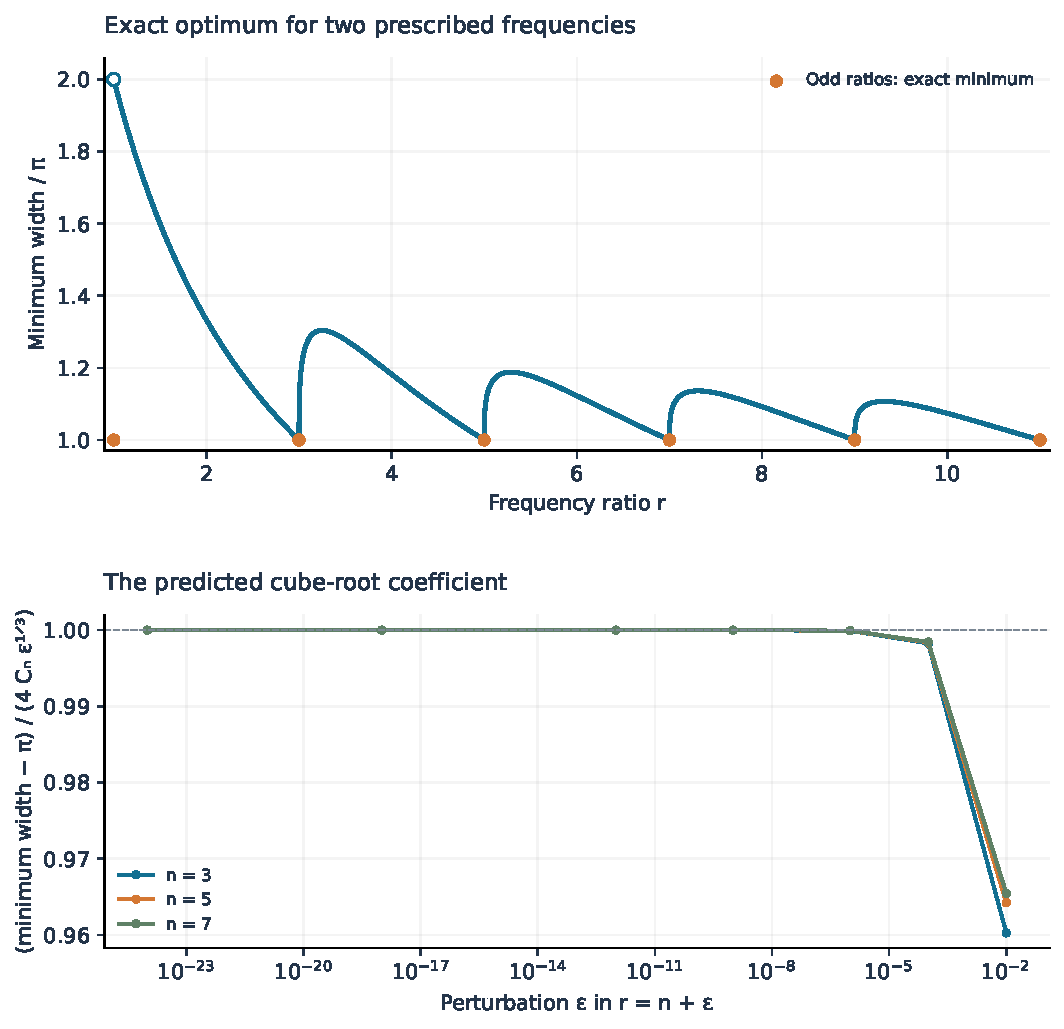
\includegraphics[width=\textwidth]{figures/filter_phase_diagram.pdf}
 \caption{The proven optimum and its resonance asymptotic, illustrated
 numerically. The values at odd ratios are exactly $\pi$. At ratio $1$
 the two constraints coincide; its value is $\pi$, although the
 right-hand limit is $2\pi$. In the second panel, the normalized excess
 tends to one as predicted by Theorem~\ref{filt:cusp}. This figure is
 generated from the supplied script, not from a source image.}
 \label{fig:phase}
\end{figure}

\subsection{What the executable checks establish}

The proof is analytic. The accompanying computations are consistency
checks aimed at arithmetic errors, incorrect signs and incorrect leading
constants. The Python files state their own scope.

\begin{center}
\small
\begin{tabular}{@{}p{.27\linewidth}p{.63\linewidth}@{}}
\toprule
Artifact & Result and limitation\\
\midrule
\texttt{filter\_checks.py} & 19 frequency-ratio examples satisfy the two
moments to better than $2\cdot10^{-85}$ in the recorded run. The
nonnegative certificate was also sampled. Numerical sampling is not
a proof of positivity.\\[4pt]
Linear programs & Ten ratio cases were discretized on
4001 nodes. The solver returned no feasible solution below the optimum
and a feasible solution above it. Discretized feasibility is only a
cross-check.\\[4pt]
\texttt{cusp.csv} & 28 high-precision cases for odd ratios
$3,5,7,11$ check the cube-root coefficient and the limiting inner mass
$2/3$.\\[4pt]
\texttt{real\_weight\_checks.py} & Exact arithmetic in
$\mathbb Q(\sqrt2)$ verifies 65 telescoping identities and recovers
13 target multiplicities, including zeros, asymmetric pairs and repeated
atoms. One fixture forces three rejected stopping points.\\[4pt]
Two-center obstruction & 364 exact queries check the two periodic
counterexample spectra, and an irrational third center distinguishes
them. The general proof is Proposition~\ref{rw:prop:reflection}.\\
\bottomrule
\end{tabular}
\end{center}

The results are preserved in machine-readable JSON and CSV. They are
reproduced by running, from the archive directory,
\begin{verbatim}
python3 scripts/filter_checks.py
python3 scripts/real_weight_checks.py \
  --output results/real_weight_checks.json
latexmk -pdf -interaction=nonstopmode -halt-on-error report.tex
\end{verbatim}
The exact reconstruction script needs only the Python standard library.
The filter script additionally needs \texttt{mpmath}, \texttt{numpy},
\texttt{scipy} and \texttt{matplotlib}. The PDF is compiled from the
included LaTeX source and bibliography. No repository access is needed
to reproduce these examples or rebuild this note.

\subsection{Proof review and a route to formal verification}

The source analysis and both new proofs were checked in separate review
passes during this AI-assisted research session. This is not external
peer review. No substantive gap was identified in those passes. The
verification notes preserve the checked signs, conductor-uniform error
bound, infinite-sum argument, reflection scope and exact-oracle
qualification. The following are the main modules for a future Lean
formalization; they are a plan, not implemented declarations.

\begin{enumerate}
\item \emph{Positive arithmetic encoder.} Formalize the multiquadratic
separation lemma and its effective tail construction. Obtain the shifted
first-Riesz explicit formula uniformly in the conductor. Prove the
Fourier--Bohr autocorrelation identity for absolutely summable frequency
families, including collisions. Combine it with integer decoding and
the discrete reflection/Pell argument. Only the explicit-formula module
uses Dirichlet GRH.
\item \emph{Two-frequency optimum.} Formalize the derivative of
$s\cos(ru)/\cos u$, its last positive lobe, and the unique outer root.
Use the nonnegative certificate to restrict the support of every
admissible measure. Finite-dimensional linear algebra gives unique
weights without an assumed symmetry. Formalize the scaled analytic
implicit-function argument to obtain the cube-root law with its
remainder. The shortening proof uses a perturbed certificate and an
explicit competing measure.
\end{enumerate}

The new results here have complete ordinary mathematical proofs, but no
claim is made that they have been accepted by Lean. The upstream GRH
formalization remains an external, separately checked input.

\subsection{Further questions suggested by the two results}

The real encoder deliberately trades numerical conditioning for exact
identifiability. A useful next question is whether a finite family of
bounded-conductor characters admits one positive real weight with
quantitative finite-time reconstruction guarantees under explicit
separation assumptions, or with a weaker metric that tolerates clusters.
The present proof supplies the exact target and separates reflection
ambiguity from coefficient decoding.

For positive cancellation, three arbitrary noncommensurate frequencies
produce a higher-dimensional moment curve. Determining its minimum
width, all support transitions and the possible fractional powers at
resonances would extend the two-frequency theorem. Requiring vanishing
jets at both frequencies is another problem: the simple cancellation
proved here does not automatically supply derivative cancellation.

\begingroup
\raggedright
\bibliographystyle{plain}
\bibliography{references}
\endgroup
\end{document}
